
%(BEGIN_QUESTION)
% Copyright 2006, Tony R. Kuphaldt, released under the Creative Commons Attribution License (v 1.0)
% This means you may do almost anything with this work of mine, so long as you give me proper credit

Complete the calibration table for this flow-measuring loop, consisting of an orifice plate, $\Delta$P transmitter, square root extractor, and indicator.  Assume the following instrument ranges:

$$\includegraphics[width=15.5cm]{i00693x01.eps}$$

\begin{itemize}
\item{$\bullet$} FE: 0-2000 l/min, 0-320 cmWC $\Delta$P
\item{$\bullet$} FT: 0-320 cmWC in, 0.2-1 bar out (linear)
\item{$\bullet$} FY: 0.2-1 bar in and out (square-root)
\item{$\bullet$} FI: 0.2-1 bar in, 0-200 l/min indication
\medskip

% No blank lines allowed between lines of an \halign structure!
% I use comments (%) instead, so that TeX doesn't choke.

$$\vbox{\offinterlineskip
\halign{\strut
\vrule \quad\hfil # \ \hfil & 
\vrule \quad\hfil # \ \hfil & 
\vrule \quad\hfil # \ \hfil & 
\vrule \quad\hfil # \ \hfil & 
\vrule \quad\hfil # \ \hfil & 
\vrule \quad\hfil # \ \hfil \vrule \cr
\noalign{\hrule}
%
% First row
Flow rate & Percent of & Orifice $\Delta$P & FT output & FY output & FI indication \cr
%
% Another row
(l/min) & max. flow (\%) & (cmWC) & signal (bar) & signal (bar) & (l/min) \cr
%
\noalign{\hrule}
%
% Another row
 & 0 &   &   &   &  \cr
%
\noalign{\hrule}
%
% Another row
  & 10 &   &   &   &  \cr
%
\noalign{\hrule}
%
% Another row
  & 25 &   &   &   &  \cr
%
\noalign{\hrule}
%
% Another row
 & 50 &   &   &   &  \cr
%
\noalign{\hrule}
%
% Another row
  & 75 &   &   &   &  \cr
%
\noalign{\hrule}
%
% Another row
  & 90 &   &   &   &  \cr
%
\noalign{\hrule}
%
% Another row
 & 100 &   &   &   &  \cr
%
\noalign{\hrule}
} % End of \halign 
}$$ % End of \vbox

\underbar{file i00693}
%(END_QUESTION)





%(BEGIN_ANSWER)

% No blank lines allowed between lines of an \halign structure!
% I use comments (%) instead, so that TeX doesn't choke.

$$\vbox{\offinterlineskip
\halign{\strut
\vrule \quad\hfil # \ \hfil & 
\vrule \quad\hfil # \ \hfil & 
\vrule \quad\hfil # \ \hfil & 
\vrule \quad\hfil # \ \hfil & 
\vrule \quad\hfil # \ \hfil & 
\vrule \quad\hfil # \ \hfil \vrule \cr
\noalign{\hrule}
%
% First row
Flow rate & Percent of & Orifice $\Delta$P & FT output & FY output & FI indication \cr
%
% Another row
(l/min) & max. flow (\%) & (cmWC) & signal (bar) & signal (bar) & (l/min) \cr
%
\noalign{\hrule}
%
% Another row
0 & 0 & 0 & 0.2 & 0.2 & 0 \cr
%
\noalign{\hrule}
%
% Another row
200 & 10 & 3.2 & 0.208 & 0.280 & 200 \cr
%
\noalign{\hrule}
%
% Another row
500 & 25 & 20 & 0.250 & 0.400 & 500 \cr
%
\noalign{\hrule}
%
% Another row
1000 & 50 & 80 & 0.400 & 0.6 & 1000 \cr
%
\noalign{\hrule}
%
% Another row
1500 & 75 & 180 & 0.650 & 0.8 & 1500 \cr
%
\noalign{\hrule}
%
% Another row
1800 & 90 & 295.2 & 0.848 & 0.920 & 1800 \cr
%
\noalign{\hrule}
%
% Another row
2000 & 100 & 320 & 1.00 & 1.00 & 2000 \cr
%
\noalign{\hrule}
} % End of \halign 
}$$ % End of \vbox


%(END_ANSWER)





%(BEGIN_NOTES)

%INDEX% Calibration: table, flow transmitter
%INDEX% Measurement, flow: calibration table

%(END_NOTES)


